\documentclass[12 pt]{article}
\usepackage[english]{babel}
\usepackage[utf8x]{inputenc}
\usepackage{graphicx}
\usepackage{caption}
\usepackage{subcaption}
\usepackage[colorinlistoftodos]{todonotes}
\usepackage{float}
\usepackage{hyperref}
\usepackage{listings}
\usepackage{enumitem}
\usepackage{xcolor}
%\usepackage{fancyhdr}
%\pagestyle{fancy}
\usepackage{amsmath, mathtools}
\usepackage[extrafootnotefeatures]{xepersian}
\usepackage{verbatim}
\date{\today}
\settextfont{XB Zar}
\setlatintextfont{Times New Roman}
\defpersianfont\RedNazanin[Color=blue]{XB Zar}
\begin{document}
	
	\begin{titlepage}
		\newcommand{\HRule}{\rule{\linewidth}{0.5mm}} 
		\center 
		\begin{figure}[H]
			\centering
			
\includegraphics[height=0.3\linewidth, width = 0.3\linewidth]{a.png}
		\end{figure}
		\textsc{\LARGE دانشگاه صنعتی شریف}\\[1.5cm] 
		%\textsc{\Large دانشکده مهندسی کامپیوتر}\\[0.5cm]
		\HRule \\[0.4cm]
		{ \huge \bfseries گزارش پروژه درس مبانی علوم اعصاب}\\[0.4cm]
		\HRule \\[1.5cm]
		\begin{minipage}{0.6\textwidth}
			\begin{center} \large
				
				علیرضا اکبری  ۹۵۱۰۵۳۷۹
			\end{center}
		\end{minipage}		
		\vfill 
	\end{titlepage}
\section*{قسمت اول}
\subsection*{1}
هدف این پژوهش پیدا کردن تعدادی  feature مربوط در تحریک تصویری ورودی است . طبق تعریف این پژوهش feature مربوط به ویژگی‌هایی از تحریک ورودی گفته می‌شود که باعث اسپایک زدن نورون‌های پیچیده می‌شود.  در واقع تاثیر بسزایی در اسپایک زدن آن دارند. برخلاف  
\lr{Null feature}
که سهمی در اسپایک زدن نورون ایفا نمی‌کنند.
در واقع  در کارهای قبلی پیدا کردن feature مربوط  در سلول‌های ساده با روش  
\lr{spike-triggered-average}
قابل انجام بوده است چرا که سلول‌ ساده رابطه خطی با تحریک ورودی دارد در حالی که سلول پیچیده با تحریک ورودی رابطه غیرخطی دارد و از روش گفته شده نمی‌توان برای آنالیز استفاده کرد . در این پژوهش از روش 
\lr{Spike-triggerd Correlation}
برای تحلیل و پیدا کردن ویژگی‌های مربوط و نامربوط تحریک تصویری ورودی استفاده شده است.
\subsection*{2}
تعریفی که از سلول پیچیده در درس دیدیم ، این بود که یک سلول پیچیده سلولی است که از کنار هم قرار گرفتن چند سلول ساده تشکیل شده است.. و این سلول ناحیه on و off خاصی ندارد ولی به حرکت حساسند. یعنی اگر تحریک حرکت کند اسپایک می‌زنند.\\
تعریفی که در مقاله ارائه شده است ، سلول‌هایی هستند که که رابطه پاسخ آن‌ها با تحریک ورودی غیرخطی است و با روش
\lr{spike-triggered-average}
نمی‌توان 
\lr{feature}
های مربوط آن را پیدا کرد. پس این سلول‌ها با معیار رابطه غیرخطی پاسخ با تحریک ورودی انتخاب می‌شوند. 
\subsection*{3}
تحریک تصویری که موجب اسپایک در نورون‌ها شده‌اند ، توزیع متفاوتی از توزیع کل تحریک خواهد داشت که این تفاوت در توزیع منجر به تفاوت در 
\lr{Moment}
های آن می‌شود. مقاله توضیح می‌دهد که اینجا از روش PCA استفاده نکرده است چرا که PCA مولفه‌ها و 
\lr{feature}
هایی
 را پیدا می‌کند که بیشترین واریانس را دارد در حالی که ما به دنبال 
 \lr{feature}
 های مربوط هستیم. \\
 در اینجا همان‌طور که گفته شد از روش 
 \lr{spike triggered correlation}
 استفاده شده است. در این روش یک ماتریس correlation به اندازه 
 $256\times 256$
 ساخته شده است که درایه 
 \lr{(i, j)}
 نشان‌دهنده correlation میان پیکسل i با j در تحریک تصویری ورودی در زمان زدن اسپایک نورون است.(تحریک تصویری ورودی یک ماتریس 
 $16\times 16$
 است که در مجموع ۲۵۶ پیکسل دارد
 )
 .این ماتریس بدین صورت پر می‌شود:
 \begin{align*}
 C_{m,n} = \frac{1}{N} \sum_{i=1}^{N} S_m(i)S_n(i)
 \end{align*}
 که N تعداد اسپایک در یک آزمایش و 
 $S_m(i)$
 و 
 $S_n(i)$
 مقادیر تحریک تصویری ورودی در هنگام آن اسپایک خاص هستند.(یک ماتریس 
 $16\times 16 $
 است که می‌توان آنرا مانند یک بردار ۲۵۶ عضوی نگاه کرد
 ).\\
 در ادامه می‌بایست ماتریسی به نام ماتریس کنترل ساخته شود. ماتریسی که پیش از این ساختیم ماتریسی بود که بر اساس زمان‌های اسپایک‌ نورون ساخته شده بود. حال برای آنکه معنادار بودن این ماتریس را بسنجیم، نیاز داریم که ماتریسی تصادفی داشته باشیم که لزوما بر اساس زمان‌های اسپایک نورون بوجود نیامده باشد و رندوم تولید شده باشد.  ساختن ماتریس کنترل هم همانند ساختن ماتریس correlation است و تعداد همان N است، اما دیگر تحریک تصویری ورودی براساس اسپایک نورون انتخاب نمی‌شود و بر اساس یک عدد رندوم ،‌ تحریک مشخص می‌شود و ماتریس کنترل شکل می‌گیرد. توضیحات سوال بعدی نیز در ادامه این سوال قرار می‌گیرد
 \subsection*{4}
 تحریک‌هایی که موجب به اسپایک شده‌اند در ماتریس correlation و تحریک‌های کلی و مستقل در ماتریس کنترل قرار می‌گیرند.نحوه ساختن این دو ماتریس را توضیح دادیم. برای مقایسه این دو ، روش مقاله بدین صورت است که تعدادی ماتریس کنترل بوجود می‌آورد و بر اساس آن، یک بازه اطمینان بوجود می‌آورد. حال مقادیر ویژه ماتریس correlation را بدست می‌آورد. بردارهای ویژه متناظر با مقادیر ویژه‌ای که به طور معناداری با بازه اطمینان کنترل تفاوت دارند ، همان feature است که در هدف مقاله به دنبال آن بوده‌ایم.
 \subsection*{5}
 نتایج آزمایش بدین صورت بوده است که برای اکثر سلول‌های پیچیدده( ۴۷ از ۶۰) دو بردار ویژه بامعنا از ماتریس کوریلیشن پیدا شده است که این دو نشان‌دهنده نواحی مکانی on و off
 \lr{receptive field}
 می‌باشند. در سه سلول تنها یک بردار ویژه بامعنا پیدا شده است که نشان‌دهنده 
 \lr{receptive field}
 برای سلول ساده است. در بقیه موارد بیش از دو بردار ویژه بامعنا پیدا شده است.\\
 همچنین در حالت دو بردا ویژه بامعنا ، با فیت کردن تابع Gabor مشاهده شده است که آن‌ها فرکانس مکانی مشابهی دارند اما با اختلاف فاز ۹۰ درجه. اما در مقاله اشاره شده است که این لزوما به معنای متعامد بودن دو بردار ویژه نیست و به خواص پاسخگویی سلول پیچیده مرتبط است
 \section*{قسمت دوم}
 \subsection*{1}
 ابتدا سعی می‌کنیم یک فایل sa0 را با تابع 
 \lr{fget\_spk}
 بخوانیم. خروجی بدین شکل است:
 		\begin{figure}[H]
 	\centering
 	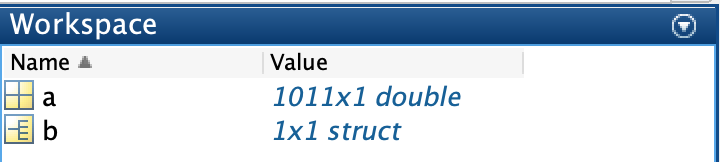
\includegraphics[height=0.2\linewidth, width = 0.5\linewidth]{b.png}
 \end{figure}
که شامل یک آرایه و یک استراکت است. آرایه زمان اسپایک نورون در آن آزمایش است. اطلاعات در استراکت بدین صورت است که دارای Fileinfo  و Datainfo است که خود نیز یک استراکت هستند که در هر یک به ترتیب اطلاعات درباره نوع فایل و نوع داده موجود است. \\
در فایل‌های log اطلاعات مربوط به تحریک ورودی در آن آزمایش وجود دارد که شامل اطلاعاتی مثل اندازه تحریک یا نام تحریک یا نرخ جابجایی فریم می‌باشد.
\subsection*{2}
کد متلب آن با اسم 
\lr{Func\_ReadData.m}
آمده است.
\subsection*{3}
دقت شود که از این قسمت به بعد ، تمام داده‌های 
\lr{msq1d.sa0}
به داده‌های csv تبدیل شدند و من و چند نفر دیگر از داده‌های csv استفاده کردیم. در ادامه کد پایتون برای سوالات نوشته شده است.\\
کد این بخش در 
\lr{Q2\_3.py}
موجود است. همچنین اسامی نورون‌های با نرخ کمتر از ۲ عبارتند از:
\lr{000413.b05
	-000720.c06
	-010801.A.b01
	-000524.c01
	-000907.f07
	-000418.a01
	-000413.b03
	-000420.b02
	-000413.b04
	-011025.A.d07
	-020213.A.i01
	-000712.b04}
\\
همچنین هیستوگرام آن بدین صورت است:
		\begin{figure}[H]
	\centering
	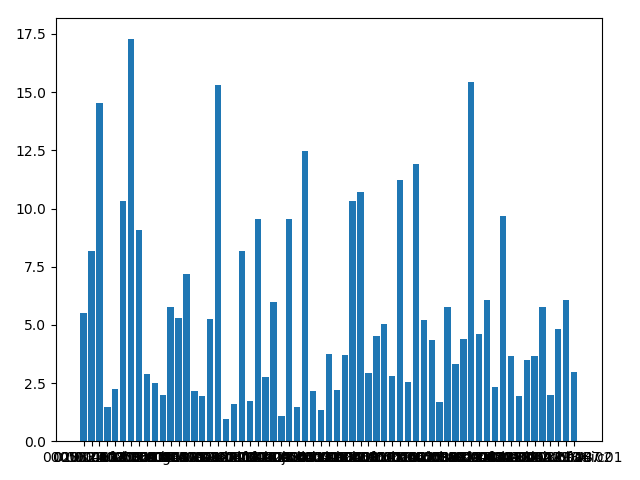
\includegraphics[height=0.5\linewidth, width = 0.7\linewidth]{c.png}
\end{figure}
\subsection*{4}
کد این بخش در 
\lr{Q2\_4.py}
موجود است.
\subsection*{5}
همان‌طور که فهمیدیم این تابع برای نشان دادن نتایج آزمایش Tune استفاده می‌شود.
در Readme مربوط به چگونگی استفاده از tview نوشته شده است که در ورژن جدید آن، فایل‌های مختلف tune دیگر مشکلی برای باز شدن ندارند و همگی آن‌ها در ورژن جدید باز می‌شوند. نحوه استفاده از این تابع بدین صورت است که آنرا صدا می‌زنیم و سپس فایل مورد نظر را باز می‌کنیم. خروجی آن برای چند نورون مختلف:

		\begin{figure}[H]
	\centering
	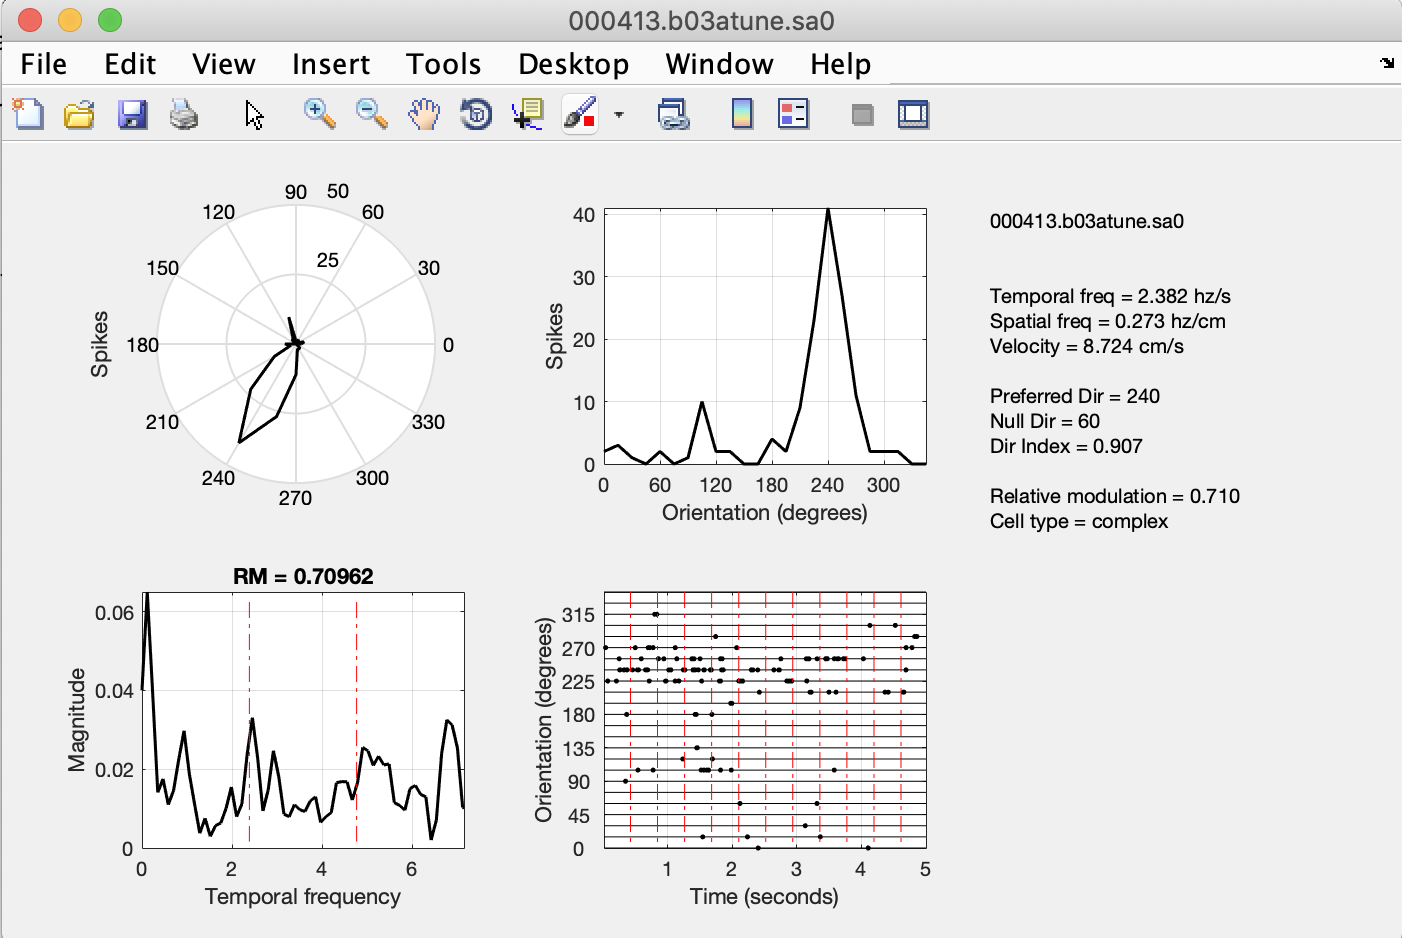
\includegraphics[height=0.5\linewidth, width = 0.7\linewidth]{d.png}
	\caption*{\lr{000413.b03atune}}
\end{figure}
		\begin{figure}[H]
	\centering
	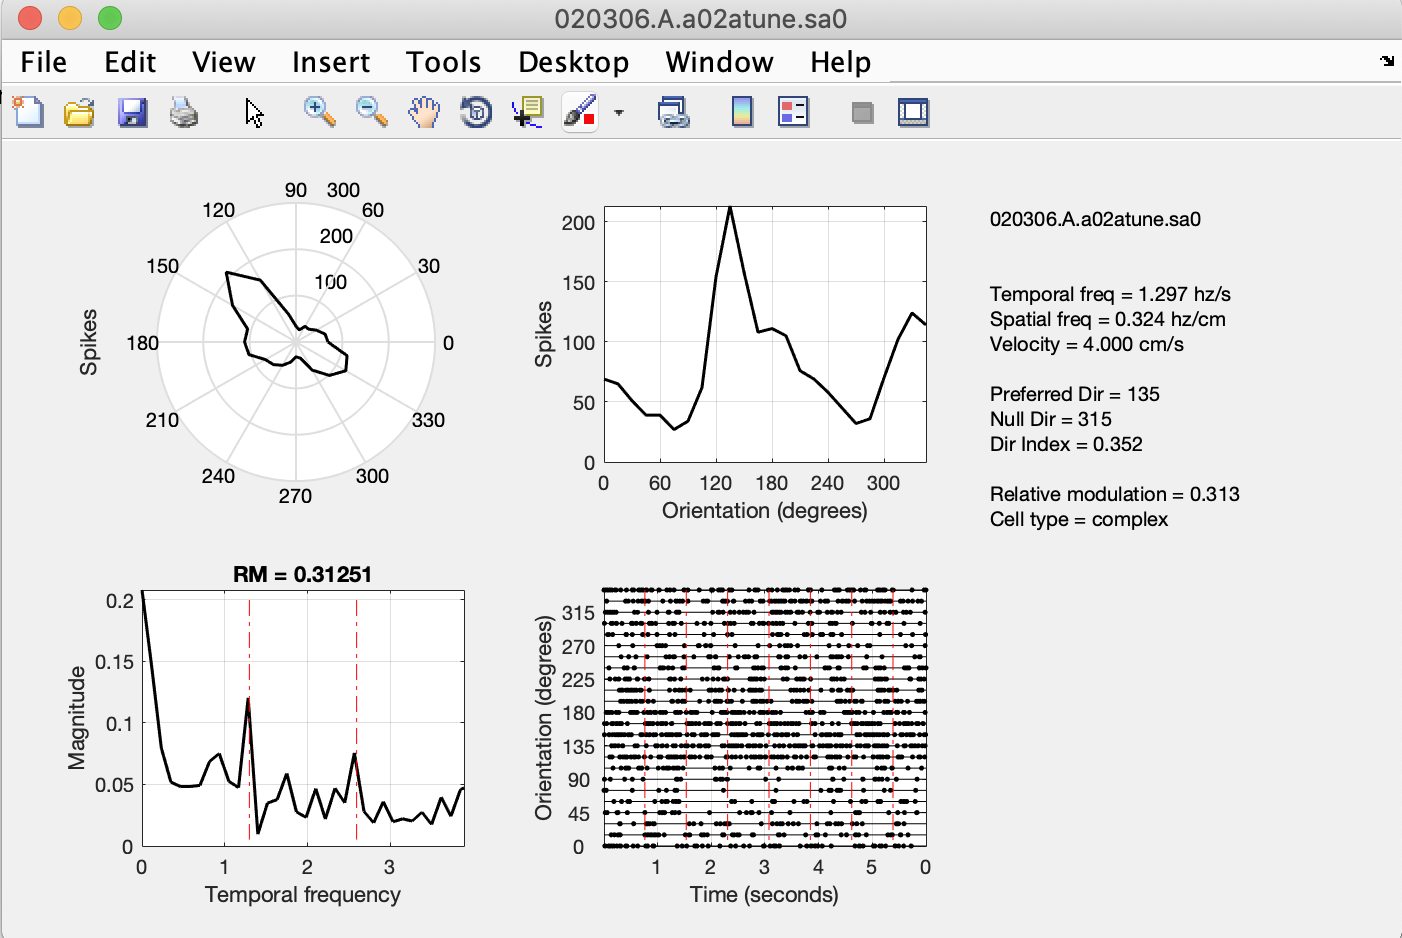
\includegraphics[height=0.5\linewidth, width = 0.7\linewidth]{e.png}
	\caption*{\lr{020306.A.a02atune}}
\end{figure}
		\begin{figure}[H]
	\centering
	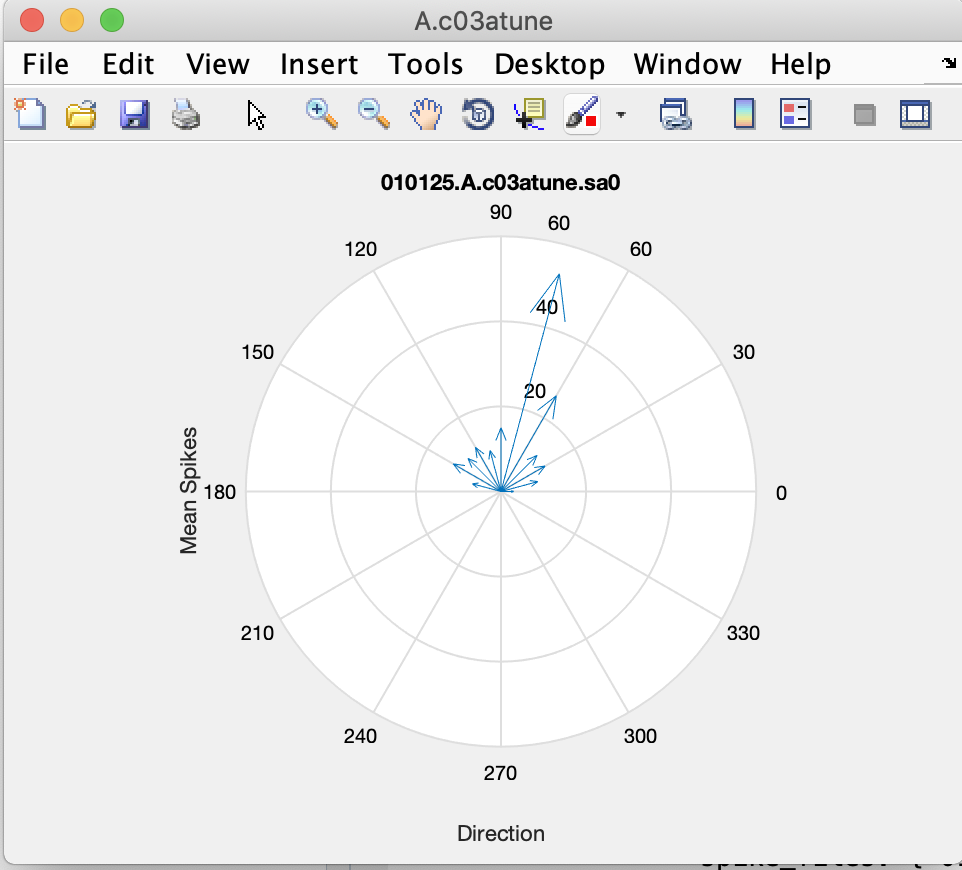
\includegraphics[height=0.5\linewidth, width = 0.7\linewidth]{f.png}
	\caption*{\lr{010125.A.c03atune}}
\end{figure}
به نظر می‌آید نحوه سازوکار tview بدین صورت است که نرخ اسپایک را در هر جهت خاص بدست می‌آورد و بیشترین نرخ را به عنوان جهت مناسب ارائه می‌دهد.
\section*{قسمت سوم}
\subsection*{1}
در 
\lr{Q3\_1.py}
موجود است
\subsection*{2}
در 
\lr{Q3\_2.py}
موجود است
\subsection*{3, 4}
در 
\lr{Q3\_3\_4.py}
موجود است. مقدار 
\lr{p-value}
محاسبه شده بسیار بامعنی است و نشان‌دهنده تفاوت میان دو توزیع را می‌دهد که یعنی این روش توانسته است توزیع اسپایک و توزیع رندوم را از یکدیگر تشخیص دهد
\subsection*{5}
در قسمت سه توانستیم توزیع projection را پیدا کنیم. حال محل تلاقی این دو توزیع را در نظر می‌گیریم و پیدا می‌کنیم که در کدام نقطه تلاقی رخ داده است. مولفه x نشان‌دهنده مقدار projection است. سطح آستانه را همین تلاقی در نظر میگیریم. یعنی اگر projection یک تصویر روی 
\lr{Spike-triggered Average}
را حساب کنیم، با توجه به سطح آستانه ، تصمیم می‌گیریم که یک تحریک معمولی دیدیم یا اسپایک. با توجه به مشاهده ، می‌خواهیم فرض کنیم واریانس دو توزیع یکسان است. پس سطح آستانه برابر است با میانگین دو میانه دو توزیع گاوسی. برای یک نورون با این ترشولد، ۵۶ درصد دسته‌بندی درست دیده می‌شود که نشان می‌ٰدهد روش خیلی خوب عمل نکرده است. کد این قسمت در همان فایل
\lr{Q3\_3\_4.py}
موجود است
\subsection*{6}
با توجه به تعداد زیاد نورون‌ها در گزارش آورده نشده است و کد آن در 
\lr{Q3\_6.py}
موجود است
\subsection*{7}
همان طور که در بخش‌های قبلی گفته شد در این روش به 
\lr{p-value}
بسیار معناداری برای جداسازی دو توزیع رسیدیم، اما دیدیم که درصد دسته‌بندی خیلی بالا نیست. همچنین در تصویرهایی که در بخش‌های قبلی تولید کردیم، نواحی خیلی واضح مانند نواحی خاموش روشن سلول‌های ساده بوجود نیامده بود که نشان می‌دهد سلول‌ها ساده نبودند.
\section*{بخش چهارم}
\subsection*{1, 3}
کد این دو قسمت در 
\lr{Q4\_1.py}
موجود است. هیستوگرام در سوال سوم برای هر یک از بردار ویژه‌ها به صورت جداگانه کشیده شده است(سه‌بعدی کشیده نشده است).  همچنین دقت شود که اجرا کد کمی طول می‌کشد.\\

\end{document}